% flashcards-title: The same twelve counters arranged two ways
% flashcards-desc: Two panels, one above the other. In panel A, twelve counters sit in three outlined loops with four counters in each loop, captioned shared equally among 3 trays. In panel B, the same twelve counters sit in four outlined loops with three counters in each loop, captioned packed into bags of 3.
\documentclass[tikz]{standalone}
\usetikzlibrary{arrows.meta,patterns}

\definecolor{qraNavy}{HTML}{17324D}
\definecolor{qraBlue}{HTML}{2B6CB0}
\definecolor{qraGold}{HTML}{B7791F}
\definecolor{qraPale}{HTML}{EAF2F8}
\definecolor{qraGray}{HTML}{5C6773}

\tikzset{
  qra axis/.style={draw=qraNavy, line width=1.2pt},
  qra tick/.style={draw=qraNavy, line width=1pt},
  qra guide/.style={draw=qraGray, densely dashed, line width=0.8pt},
  qra counter/.style={circle, draw=qraNavy, fill=qraPale, line width=0.9pt, minimum size=7mm, inner sep=0pt},
  qra label/.style={font=\sffamily\bfseries, text=qraNavy},
  qra small label/.style={font=\sffamily, text=qraNavy},
}

\begin{document}
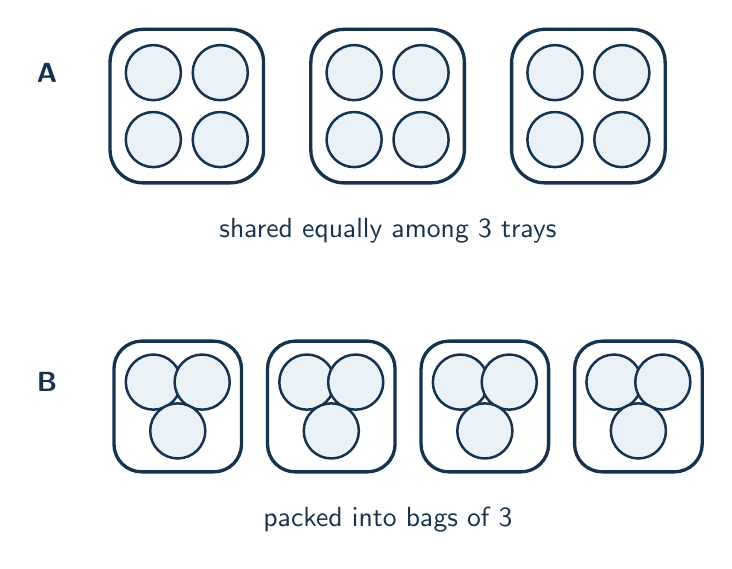
\begin{tikzpicture}
  % Panel A: three loops of four (2x2 counters each)
  \node[qra label] at (-1.35,0.85) {A};
  \foreach \g in {0,1,2} {
    \begin{scope}[xshift=\g*2.55cm]
      \node[qra counter] at (0,0) {};
      \node[qra counter] at (0.85,0) {};
      \node[qra counter] at (0,0.85) {};
      \node[qra counter] at (0.85,0.85) {};
      \draw[qra axis, rounded corners=12pt] (-0.55,-0.55) rectangle (1.4,1.4);
    \end{scope}
  }
  \node[qra small label] at (2.98,-1.15) {shared equally among 3 trays};

  % Panel B: four loops of three (3 counters in a row each)
  \begin{scope}[yshift=-3.5cm]
    \node[qra label] at (-1.35,0.42) {B};
    \foreach \g in {0,1,2,3} {
      \begin{scope}[xshift=\g*1.95cm]
        \node[qra counter] at (0,0.42) {};
        \node[qra counter] at (0.62,0.42) {};
        \node[qra counter] at (0.31,-0.2) {};
        \draw[qra axis, rounded corners=10pt] (-0.5,-0.72) rectangle (1.12,0.94);
      \end{scope}
    }
    \node[qra small label] at (2.98,-1.32) {packed into bags of 3};
  \end{scope}
\end{tikzpicture}
\end{document}
